\section{Generative Music System based on Deep Learning Transformer Model}

Amaral et al. introduced an adaptive music generation
architecture which is based on the deep learning 
Transformer model \cite{amaral2022adaptive}.
They state that their developed model has a couple of similarities
to the AMS \cite{hutMcCormAms} which was developed by Hutchings and 
McCormack \cite{amaral2022adaptive}. The similarities are the usage of
neural network techniques as well as the usage of an emotion-based model \cite{amaral2022adaptive}. The architecure itself will be explained 
in this chapter.

\subsubsection{Transformer model}

\begin{figure}[h]
    \centering
    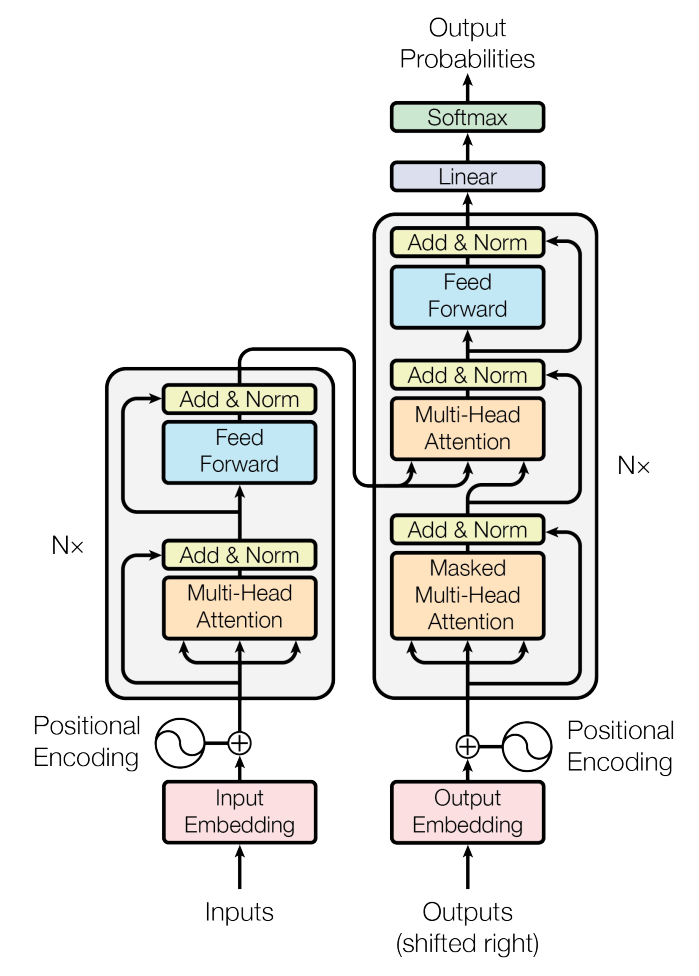
\includegraphics[height=8cm]{images/transformer_architecture.png}
    \caption{Transformer architecture \cite{vaswani2017transformer}}
    \label{fig:transformer_architecture}
\end{figure}

The authors say that their system implements the technology of the 
Transformer model used in deep learning \cite{amaral2022adaptive}. 
The Transformer architecture \cite{vaswani2017transformer} is used in 
their architecture because it is knows for its ability to enforce consistency and structure \cite{amaral2022adaptive}.

The Transformer architecture was first developed and introduced by 
Vaswani et al. It is known for its faster training time and uses attention mechanisms
to represent the dependencies of the input data. \cite{vaswani2017transformer}. 
As shown in \Cref{fig:transformer_architecture}, the
transformer architecture contains several components:

\begin{enumerate}[label=\alph*)]
    \item \emph{Encoders and decoders}:
    Encoders consist of \( N = 6 \) identical layers , in which every layer contains
    a multi-head and self-attention mechanism, which is responsible for the parallel
    observation of the input sequence and a feed-forward neural network, which is a 
    dense layer, which is applied on the output of the attention-mechanism \cite{vaswani2017transformer}. The decoder also has N identical layers, but in addition
    to the components of the encoder, it also has a second multi-head attention layer which
    pays attention the the output of the encoder \cite{vaswani2017transformer}.
    \item \emph{Attention mechanism}:
    The attention mechanism has two different types of attention function: the self-attention
    and the multi-head attention \cite{vaswani2017transformer}.
    The self-attention mechanism calculates a weighted sum of input vectors, in which
    the weights represent how much every part of the input is showing attention to the
    other part \cite{vaswani2017transformer}.
    The multi-head attention executes the self-attention mechanism multiple times parallel
    in order to learn different aspects of the input data \cite{vaswani2017transformer}.
    \item \emph{Positional encoding}:
    Due to the fact that transformer models do not take into any inherent order in the
    input, a positional encoding is added which gives information about the
    position to the token vectors \cite{vaswani2017transformer}.
    \item \emph{Residual connections and layer normalization}
    Residual connections are connections that sum up the input of a layer to its output
    to simplify the gradient flow \cite{vaswani2017transformer}. The layer normalization
    is done to increase the training stability \cite{vaswani2017transformer}.
\end{enumerate}

\subsubsection{Training of the Transformer model}

For the training, the user is able to choose its own music genre containing 
the music as he likes \cite{amaral2022adaptive}. If trained, the
music matches with the corresponding style of the user \cite{amaral2022adaptive}.
Nevertheless, the authors of the paper have used the Spotify Playlist 
named "Ambient Songs for Creativity and Calm" \cite{spotify2022ambient} 
containing approximately 20 hours of music within 
165 tracks of music \cite{amaral2022adaptive}.
The authors state that they have turned the compressed audio files (mp3)
have been transformed into wave form (wav), and from this format 
they have been transformed into MIDI files \cite{amaral2022adaptive}.
A short description to MIDI files can be found in Section~\ref{sec:ams}, 
for more details, see \cite{midi_explanation} and \cite{midi_general}.

\subsubsection{Layering of the architecture}

The authors use four layers in total in their architecture
for generating music and explain that they are doing it in \cite{stuart2019mozart}
similar to real orchestras \cite{amaral2022adaptive}.
This is how the the layer model of the authors 
Amaral et al. is organized:
\begin{itemize}
    \item layer one: the most conservative and neutral \cite{amaral2022adaptive}
    \item layer two: for more excitement, perhaps through another instrument that is involved
    \cite{amaral2022adaptive}
    \item layer three and four: layers to intensify
    immersion and tension \cite{amaral2022adaptive}
\end{itemize}

\subsubsection{Emotion model}



Similar to the AMS \cite{hutMcCormAms}, the authors of \cite{amaral2022adaptive} use an emotion model
to record the game play context, containing the game
itself and the players playing it \cite{amaral2022adaptive}.
The emotion model is the arousal/valence model from
\cite{russell1980circumplex} which uses two parameters:
the arousal, or intensity of an emotion and the valence,
or simply the quality (either positive, negative, neutral...) \cite{amaral2022adaptive}.

\begin{figure}[h]
\centering

\begin{tabular}{|l|l|l|l|}
\hline
\textbf{} & \textbf{Sad} & \textbf{Neutral} & \textbf{Happy} \\
\hline
\textbf{All Layers} & Angry & Excited & Happy \\
\hline
\textbf{Both First and Second} & Sad & Calm & Relaxed \\
\hline
\textbf{Only First} & Depressed & Sleepy & Peaceful \\
\hline
\end{tabular}
\caption{Strategy/Layer/Emotion model, with 9 pre-defined emotions based on the arousal/valence model (re-created from \cite{amaral2022adaptive})}
\label{fig:layer_emotion}

\end{figure}

For simplicity reasons, the authors decided on 9 
emotions \cite{amaral2022adaptive}. 
The used emotions and the activation of the musical
layers is shown in \Cref{fig:layer_emotion}.

\subsubsection{Architecture and implementation}
The architecture itself is implemented as a server
to serve as a service for several game clients based on game engines like Unity, Unreal, or other ones \cite{amaral2022adaptive}.

The architecture works like this according to the authors: First step is for the client to request 
music from the server \cite{amaral2022adaptive}. The Server uses the emotion model
to map the feeling using the arousal/valence parameters
from the game \cite{amaral2022adaptive}. Then, the server fetches a song from
its memory, that is related to the emotion \cite{amaral2022adaptive}. If there is
currently no song available, it will be generated by 
the transformer architecture \cite{amaral2022adaptive}. The response is delivered
with the calculated music and finally, the memory is refreshed \cite{amaral2022adaptive}.








